\documentclass{article} % For LaTeX2e
\usepackage{iclr2025,times}

\usepackage{hyperref}
\usepackage{url}
\usepackage{graphicx}
\usepackage{subfigure}
\usepackage{booktabs}

% For theorems and such
\usepackage{amsmath}
\usepackage{amssymb}
\usepackage{amsthm}

% Custom
\usepackage{multirow}
\usepackage{color}
\usepackage{colortbl}
\usepackage[capitalize,noabbrev]{cleveref}
\usepackage{xspace}

\graphicspath{{../figures/}} % DO NOT CHANGE THIS.

\begin{filecontents}{references.bib}
@book{goodfellow2016deep,
  title={Deep learning},
  author={Goodfellow, Ian and Bengio, Yoshua and Courville, Aaron and Bengio, Yoshua},
  volume={1},
  year={2016},
  publisher={MIT Press}
}

% This work discusses a compositional framework for integrating neural and symbolic systems as modular components, which is directly relevant to the methodology proposed in this paper. It will be cited in the methodology section to provide foundational context for the neural-symbolic integration approach used in the model.
@inproceedings{tsamoura2020neuralsymbolicia,
 author = {Efthymia Tsamoura and Loizos Michael},
 booktitle = {Proceedings of the AAAI Conference on Artificial Intelligence},
 pages = {5051--5060},
 title = {Neural-Symbolic Integration: A Compositional Perspective},
 volume = {34},
 number = {04},
 year = {2020}
}

% This paper discusses a neural-symbolic prompting method for complex reasoning tasks using code as intermediate steps, providing both zero-shot and few-shot versions. It is relevant to support the discussion on zero-shot reasoning capabilities and neural-symbolic integration in the methodology section of the paper.
@article{hu2023codepa,
 author = {Hanqing Hu and Haotong Yang and Zhouchen Lin and Muhan Zhang},
 journal = {arXiv preprint arXiv:2305.18507},
 title = {Code Prompting: A Neural Symbolic Method for Complex Reasoning in Large Language Models},
 year = {2023}
}

% This paper discusses zero-shot learning methodologies applied to land cover classification using convolutional neural networks. It includes an exploration of feature extraction, class signature prediction, and evaluation metrics such as precision and F1-score. This is relevant to the methodology and experiment sections of the paper, as it provides foundational insights into zero-shot learning frameworks and evaluation strategies.
@article{pradhan2020unseenlc,
 author = {Pradhan, Biswajeet and Al-Najjar, Hassan and Sameen, Muhammad Imran and Tsang, Irene and Al-Amri, Mohammed},
 journal = {Remote Sensing},
 pages = {1676},
 title = {Unseen Land Cover Classification from High-Resolution Orthophotos Using Integration of Zero-Shot Learning and Convolutional Neural Networks},
 volume = {12},
 number = {10},
 year = {2020}
}

% The KANDY Benchmark provides a framework for symbolic reasoning tasks inspired by Kandinsky patterns, focusing on compositionality and continual learning. This work is relevant for discussing the context and importance of benchmarks like SPR_BENCH in symbolic reasoning evaluation and will be cited in the experiments section to provide background on symbolic reasoning benchmarks.
@article{lorello2024thekb,
 author = {Lorello, Luca Salvatore and Lippi, Marco and Melacci, Stefano},
 journal = {Machine Learning},
 pages = {161},
 title = {The KANDY Benchmark: Incremental Neuro-Symbolic Learning and Reasoning with Kandinsky Patterns},
 volume = {114},
 number = {6},
 year = {2024}
}

% This paper proposes a neural-symbolic framework based on statistical relational learning (NSF-SRL) and evaluates its generalization performance on zero-shot learning tasks. It discusses the integration of deep learning with symbolic reasoning and provides insights into evaluation strategies. This is relevant for the methodology and experiments sections of the paper, particularly in discussing neural-symbolic frameworks and their evaluation metrics for zero-shot learning tasks.
@article{yu2023ann,
 author = {Yu, Dongran and Liu, Xueyan and Pan, Shirui and Li, Anchen and Yang, Bo},
 journal = {arXiv preprint arXiv:2309.08931},
 title = {A Novel Neural-symbolic System Under Statistical Relational Learning},
 year = {2023}
}
\end{filecontents}

\title{Challenges in Zero-Shot Synthetic PolyRule Reasoning via Neural-Symbolic Integration}

\author{Anonymous Authors}

\begin{document}

\maketitle

\begin{abstract}
We investigate the integration of neural networks with symbolic reasoning frameworks for zero-shot learning in Synthetic PolyRule Reasoning~(SPR). Despite the theoretical potential of neural-symbolic models to generalize to unseen rules without retraining, our experiments reveal significant challenges in achieving this generalization. Evaluating on the SPR\_BENCH benchmark, we observe that conventional neural models tend to overfit training data and struggle with zero-shot reasoning on unseen rules. These findings underscore the need for more robust neural-symbolic integration methods to enable effective zero-shot reasoning in SPR tasks.
\end{abstract}

\section{Introduction}
\label{sec:intro}

Zero-shot learning is a critical capability for artificial intelligence systems, enabling models to generalize to unseen classes or rules without additional training~\cite{pradhan2020unseenlc}. In the context of symbolic reasoning, integrating neural networks with symbolic frameworks presents a promising approach to achieve this capability~\cite{tsamoura2020neuralsymbolicia}. Synthetic PolyRule Reasoning~(SPR) represents a challenging domain where models must infer and apply complex, unseen rules to sequences of symbols, mimicking aspects of human reasoning.

In this work, we explore the integration of neural networks with symbolic reasoning frameworks to achieve zero-shot learning in SPR. While neural-symbolic models theoretically possess the capacity for such generalization, our experiments reveal substantial challenges. Specifically, we find that traditional neural approaches often overfit the training data and lack the ability to generalize to sequences governed by unseen rules.

Our study implements a neural-symbolic model designed for zero-shot learning in SPR. We conduct a comprehensive evaluation on the SPR\_BENCH benchmark~\cite{lorello2024thekb}, analyzing the model's performance using Shape-Weighted Accuracy~(SWA), Color-Weighted Accuracy~(CWA), and the PolyRule Harmonic Accuracy~(PHA) metrics. We identify and discuss key challenges in generalization and overfitting inherent in the integration of neural networks with symbolic reasoning frameworks for zero-shot SPR.

These findings highlight the limitations of current neural-symbolic integration methods and suggest directions for future research to enhance zero-shot reasoning capabilities in complex symbolic domains like SPR.

\section{Related Work}
\label{sec:related}

Zero-shot learning enables models to classify unseen classes or apply new rules without additional training~\cite{pradhan2020unseenlc}. Neural-symbolic integration combines neural networks' learning capabilities with symbolic systems' reasoning abilities~\cite{tsamoura2020neuralsymbolicia}. \citet{yu2023ann} proposed a neural-symbolic system under statistical relational learning, demonstrating potential in zero-shot tasks. For complex reasoning, \citet{hu2023codepa} introduced a neural-symbolic method leveraging code prompts in large language models. Benchmarks such as KANDY~\cite{lorello2024thekb} provide datasets for evaluating neuro-symbolic learning, analogous to SPR\_BENCH used in our experiments.

\section{Background}
\label{sec:background}

\textbf{Synthetic PolyRule Reasoning (SPR)} involves classifying sequences of symbols based on underlying symbolic rules. These rules dictate the correct classification but are not explicitly provided to the model. The SPR\_BENCH benchmark offers a dataset for training and evaluating models on SPR tasks, emphasizing the ability to infer and apply unseen rules.

\textbf{Evaluation Metrics}: We utilize Shape-Weighted Accuracy~(SWA) and Color-Weighted Accuracy~(CWA) to assess model performance. SWA weights accuracy based on the variety of shapes in the sequence, while CWA weights based on color variety. The PolyRule Harmonic Accuracy~(PHA) is the harmonic mean of SWA and CWA, providing an overall performance measure that balances both shape and color considerations.

\section{Method}
\label{sec:method}

Our approach integrates a neural network with symbolic reasoning to enable zero-shot learning in SPR. The model consists of a neural network component—a two-layer Multilayer Perceptron~(MLP)—that processes sequences of symbols. Each symbol is tokenized into shape and color components, encoded using one-hot vectors, and concatenated to form the input feature vector. The MLP aims to extract meaningful representations from these sequences.

The symbolic reasoning component leverages the neural features to infer underlying rules and make predictions. It is designed to generalize to unseen rules by utilizing the structured representations provided by the neural network.

Despite this integration, we observed significant challenges. The model performs well on training data but poorly on validation and test sets, indicating overfitting. It struggles to generalize to sequences governed by unseen rules, failing to achieve high SWA and CWA on the test set.

\section{Experiments}
\label{sec:experiments}

We conduct extensive experiments to evaluate the model's zero-shot learning capabilities in SPR.

\subsection{Experimental Setup}

We use the SPR\_BENCH dataset~\cite{lorello2024thekb}, which includes training, validation, and test splits. The test set contains sequences governed by rules not seen during training, assessing zero-shot generalization. The MLP is trained with a maximum of 50 epochs using early stopping based on the PHA metric on the validation set. We use the Adam optimizer with a learning rate of $1 \times 10^{-3}$ and apply a batch size of 32.

\subsection{Results and Analysis}

\textbf{Training Dynamics}: Figure~\ref{fig:training_results} illustrates the training and validation loss curves, as well as the PHA (PolyRule Harmonic Accuracy) over epochs. The training loss decreases steadily, indicating that the model fits the training data well. However, the validation loss plateaus and slightly increases after early epochs, suggesting overfitting. The training PHA increases, but the validation PHA remains low and stable, reinforcing the overfitting concern.

\textbf{Test Performance}: We evaluate the model on the test set containing unseen rules. The test metrics are presented in Table~\ref{tab:test_metrics}. The SWA, CWA, and PHA are approximately 0.26--0.27, indicating poor generalization to unseen rules. The significant misclassifications in the confusion matrix (see Appendix~\ref{sec:additional_results}, Figure~\ref{fig:test_confusion}) further emphasize the model's inability to generalize.

The results indicate that the neural-symbolic model lacks the ability to infer and apply unseen rules effectively. The model's performance on the training data suggests it has learned to memorize patterns present in the training set without capturing the underlying rule structures necessary for zero-shot generalization. This shortcoming is critical in tasks requiring adaptability to new, unseen scenarios.

\section{Conclusion}
\label{sec:conclusion}

Our study highlights significant challenges in achieving zero-shot learning in SPR through neural-symbolic integration. The model's inability to generalize to unseen rules without additional training underscores the limitations of traditional neural approaches in symbolic reasoning tasks.

Future work should focus on developing more robust neural-symbolic integration methods capable of capturing the compositional and rule-based nature of SPR. Incorporating explicit rule induction mechanisms, leveraging attention-based architectures, or integrating external symbolic knowledge bases may enhance zero-shot reasoning capabilities. Exploring alternative architectures that can effectively handle sequential and symbolic data might also improve generalization in SPR tasks.

\bibliography{references}
\bibliographystyle{iclr2025}

\appendix

\section*{\LARGE Appendix}

\section{Additional Experimental Results}
\label{sec:additional_results}

\subsection{Confusion Matrix}

Figure~\ref{fig:test_confusion} shows the confusion matrix for the model's predictions on the test set. The widespread misclassifications indicate that the model fails to generalize to unseen rules.

\begin{figure}[h!]
\centering
\includegraphics[width=0.6\textwidth]{baseline_test_confusion_matrix.png}
\caption{Confusion matrix for the model's predictions on the test set. Misclassifications are widespread, indicating poor generalization to unseen rules.}
\label{fig:test_confusion}
\end{figure}

\subsection{Ablation Studies}

We performed several ablation studies to investigate factors contributing to the model's poor generalization.

\subsubsection{Impact of Joint-Token Representation}

We experimented with a joint-token representation where shape and color are combined into a single token. Figure~\ref{fig:joint_token} shows that this modification did not improve performance. The model still overfits to the training data and fails to generalize, suggesting that simply altering the input representation is insufficient.

\begin{figure}[h!]
\centering
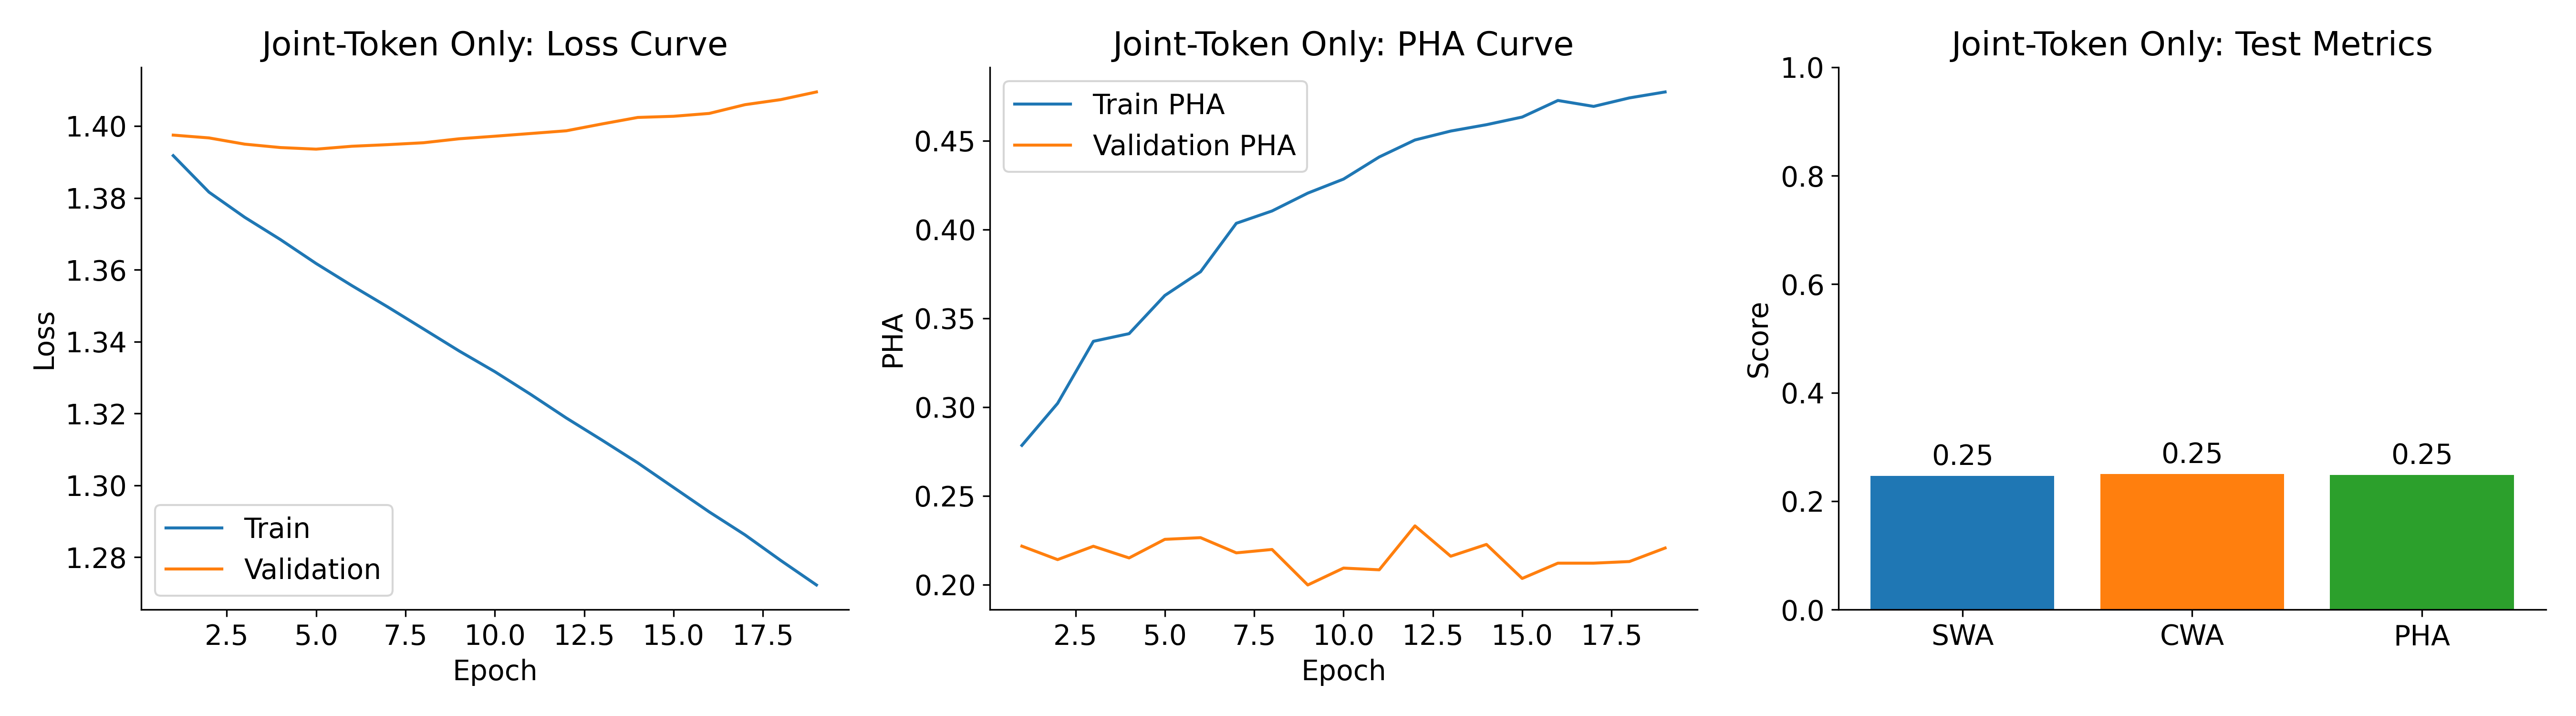
\includegraphics[width=0.6\textwidth]{joint_token_only_combined.png}
\caption{Using a joint-token representation did not enhance generalization; performance remained low with significant overfitting.}
\label{fig:joint_token}
\end{figure}

\subsubsection{Training Without Early Stopping}

Training the model without early stopping led to increased overfitting (Figure~\ref{fig:no_early_stopping}). The validation loss increased while the training loss continued to decrease, and test performance did not improve, indicating that longer training exacerbates overfitting.

\begin{figure}[h!]
\centering
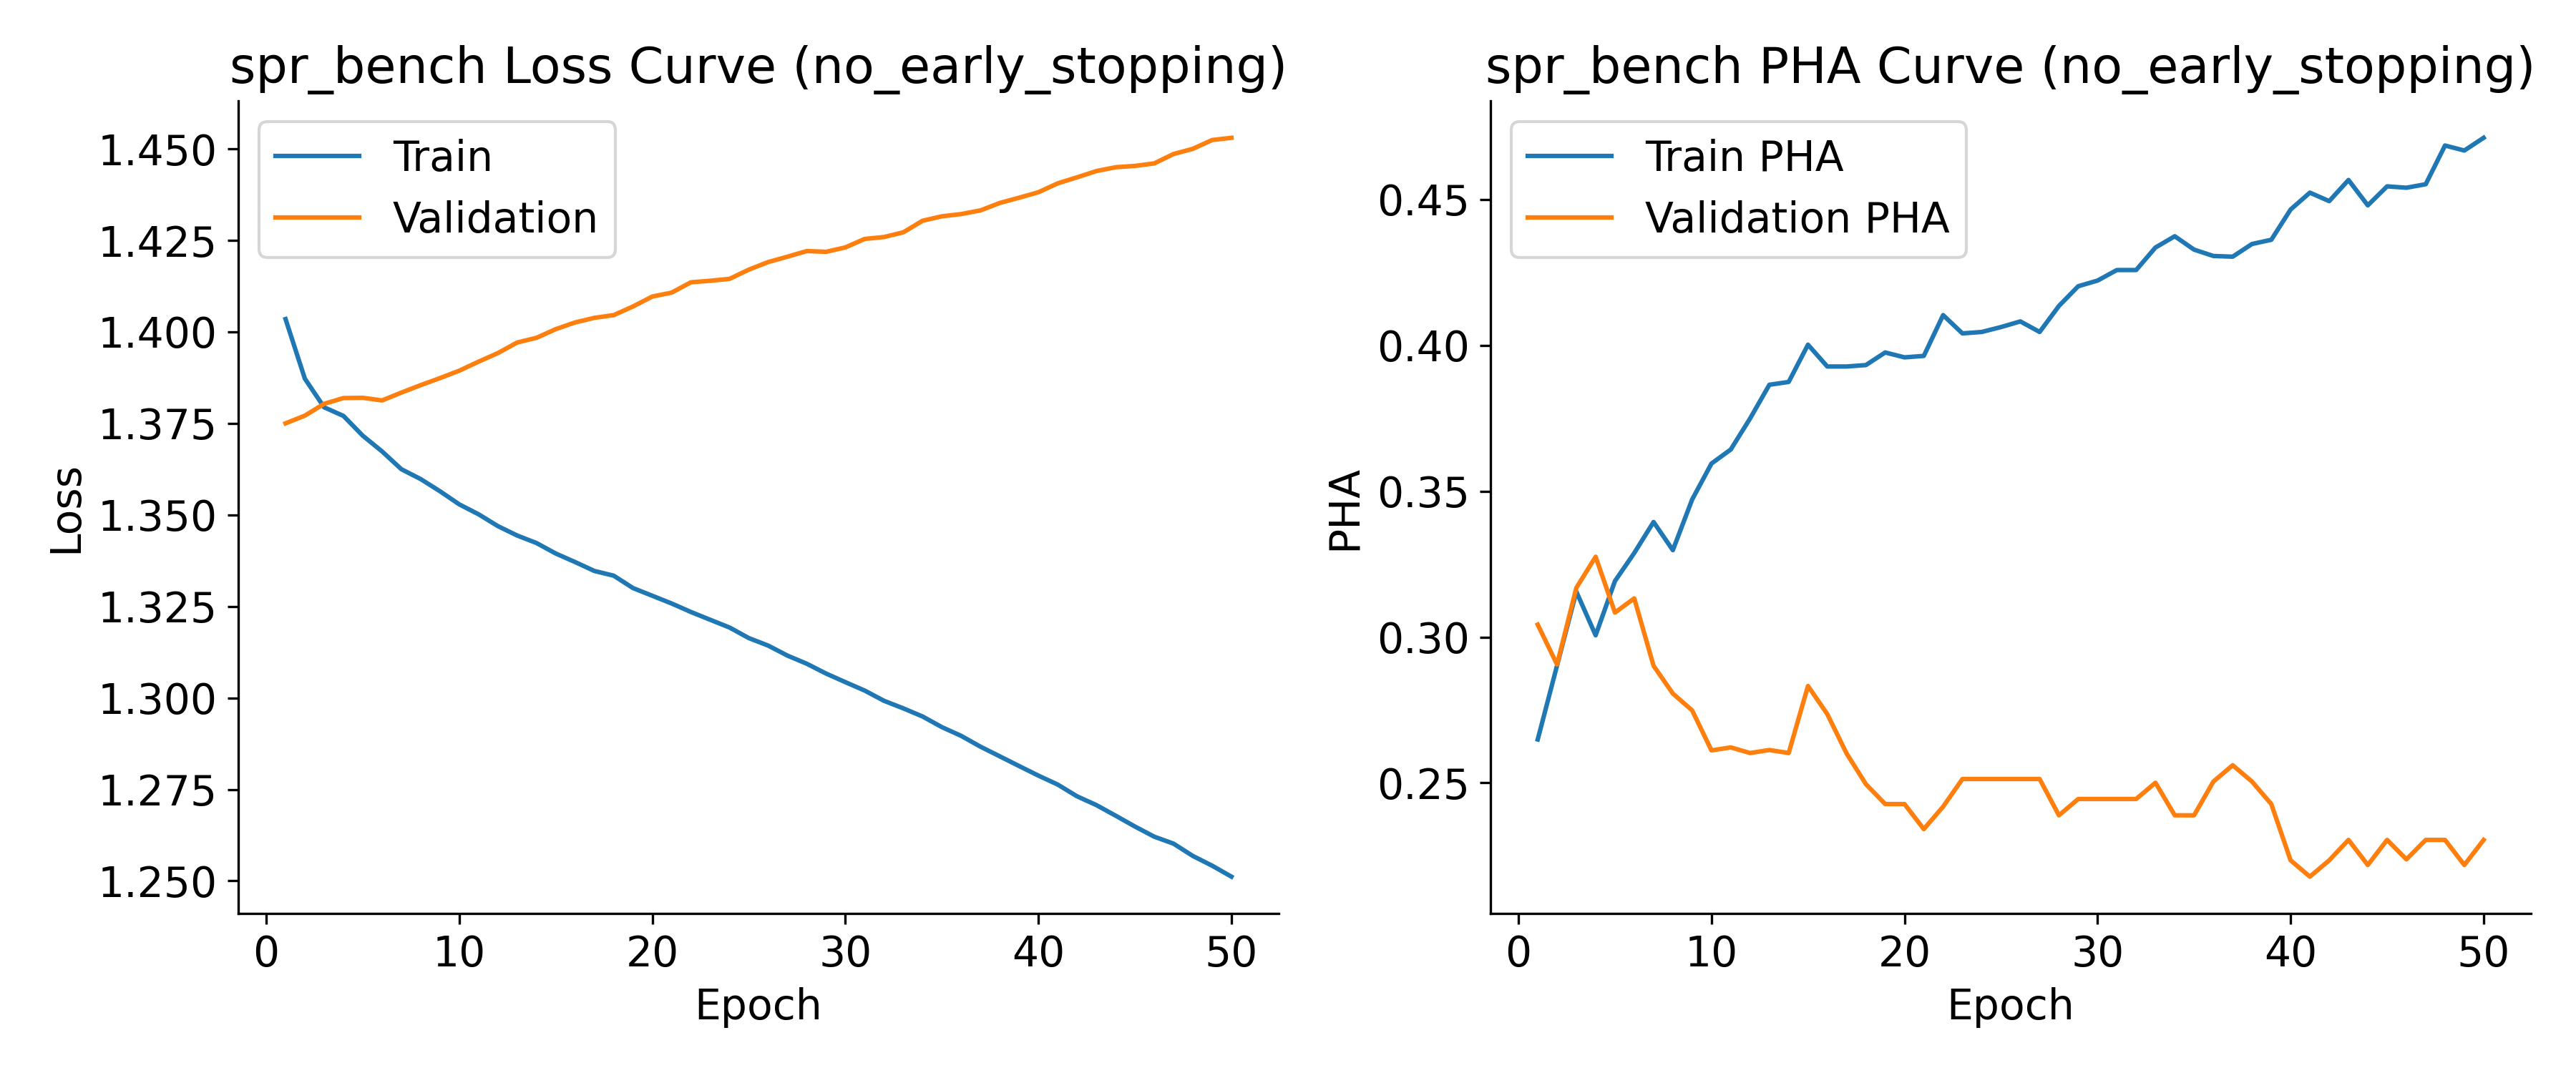
\includegraphics[width=0.6\textwidth]{spr_bench_no_early_stopping_loss_and_PHA.png}
\caption{Training without early stopping led to increased overfitting; validation loss increased while training loss decreased.}
\label{fig:no_early_stopping}
\end{figure}

\subsubsection{Feature Ablations}

Removing color features or using a linear model without hidden layers did not enhance generalization (Figures~\ref{fig:remove_color} and~\ref{fig:no_hidden_layer}). These results suggest that neither the complexity of the model nor the specific features used are the primary issues.

\begin{figure}[h!]
\centering
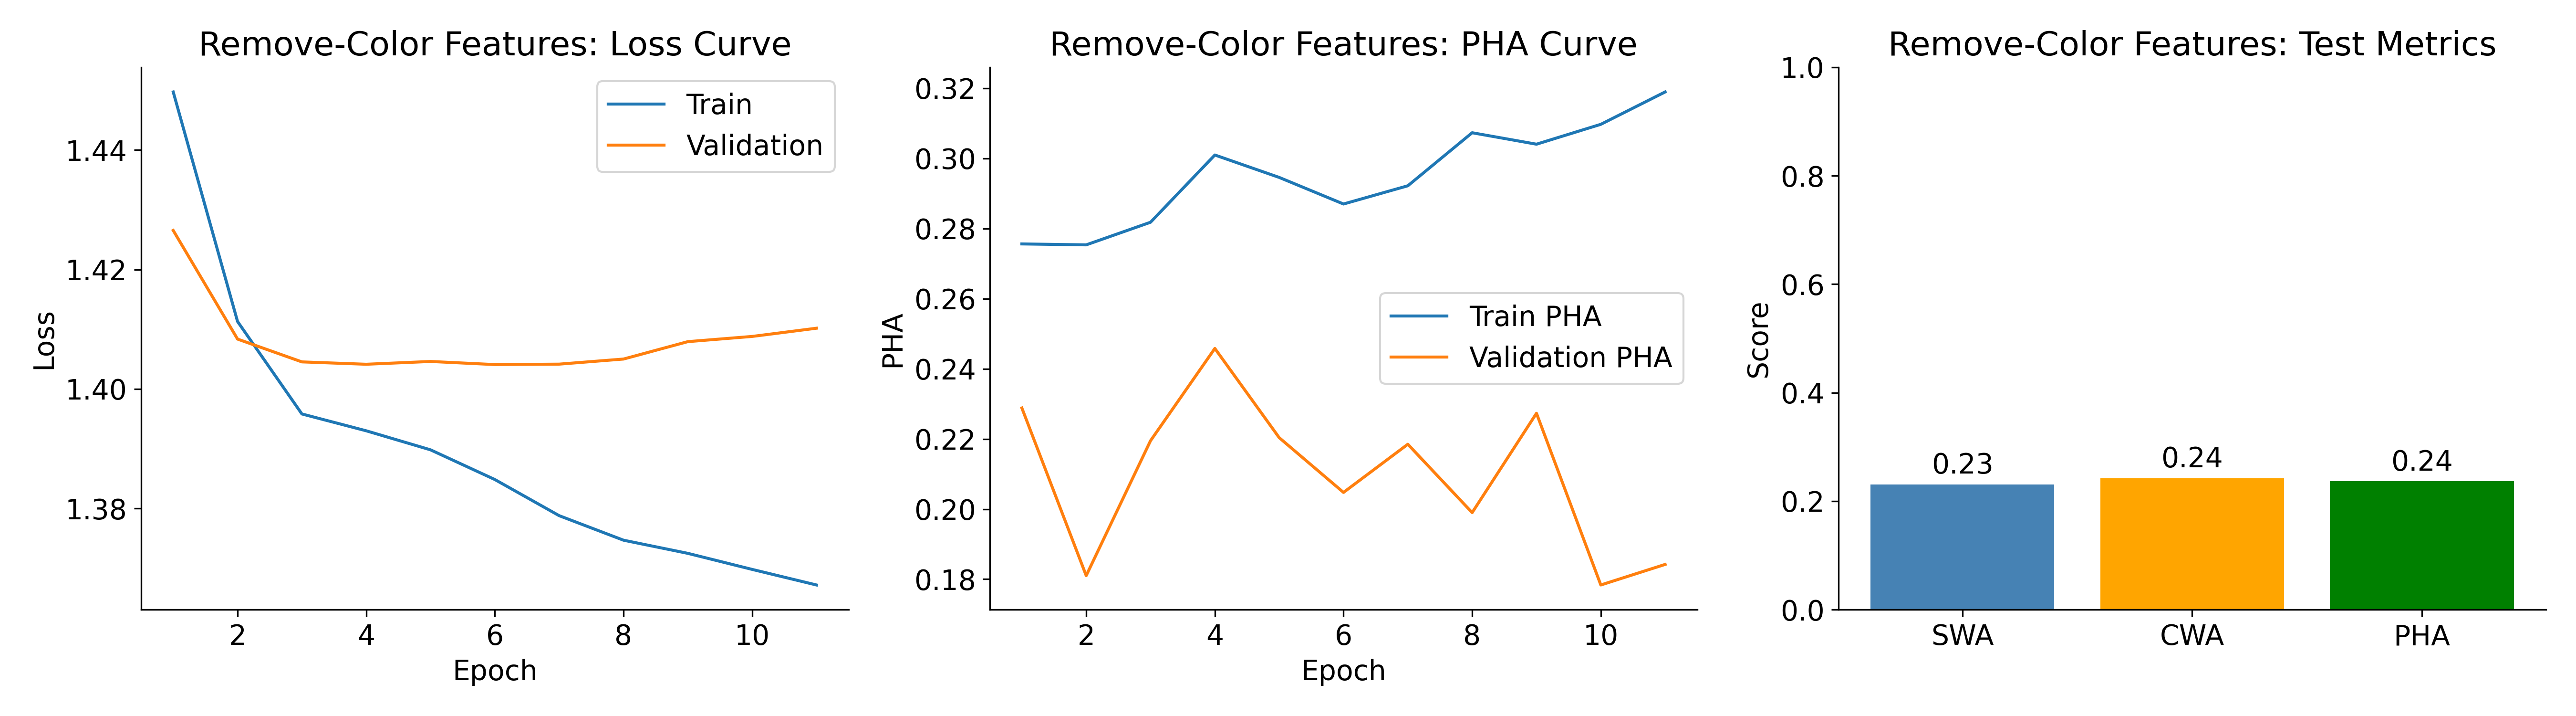
\includegraphics[width=0.6\textwidth]{remove_color_features_combined.png}
\caption{Removing color features did not improve performance, suggesting that both shape and color information are crucial for the task.}
\label{fig:remove_color}
\end{figure}

\begin{figure}[h!]
\centering
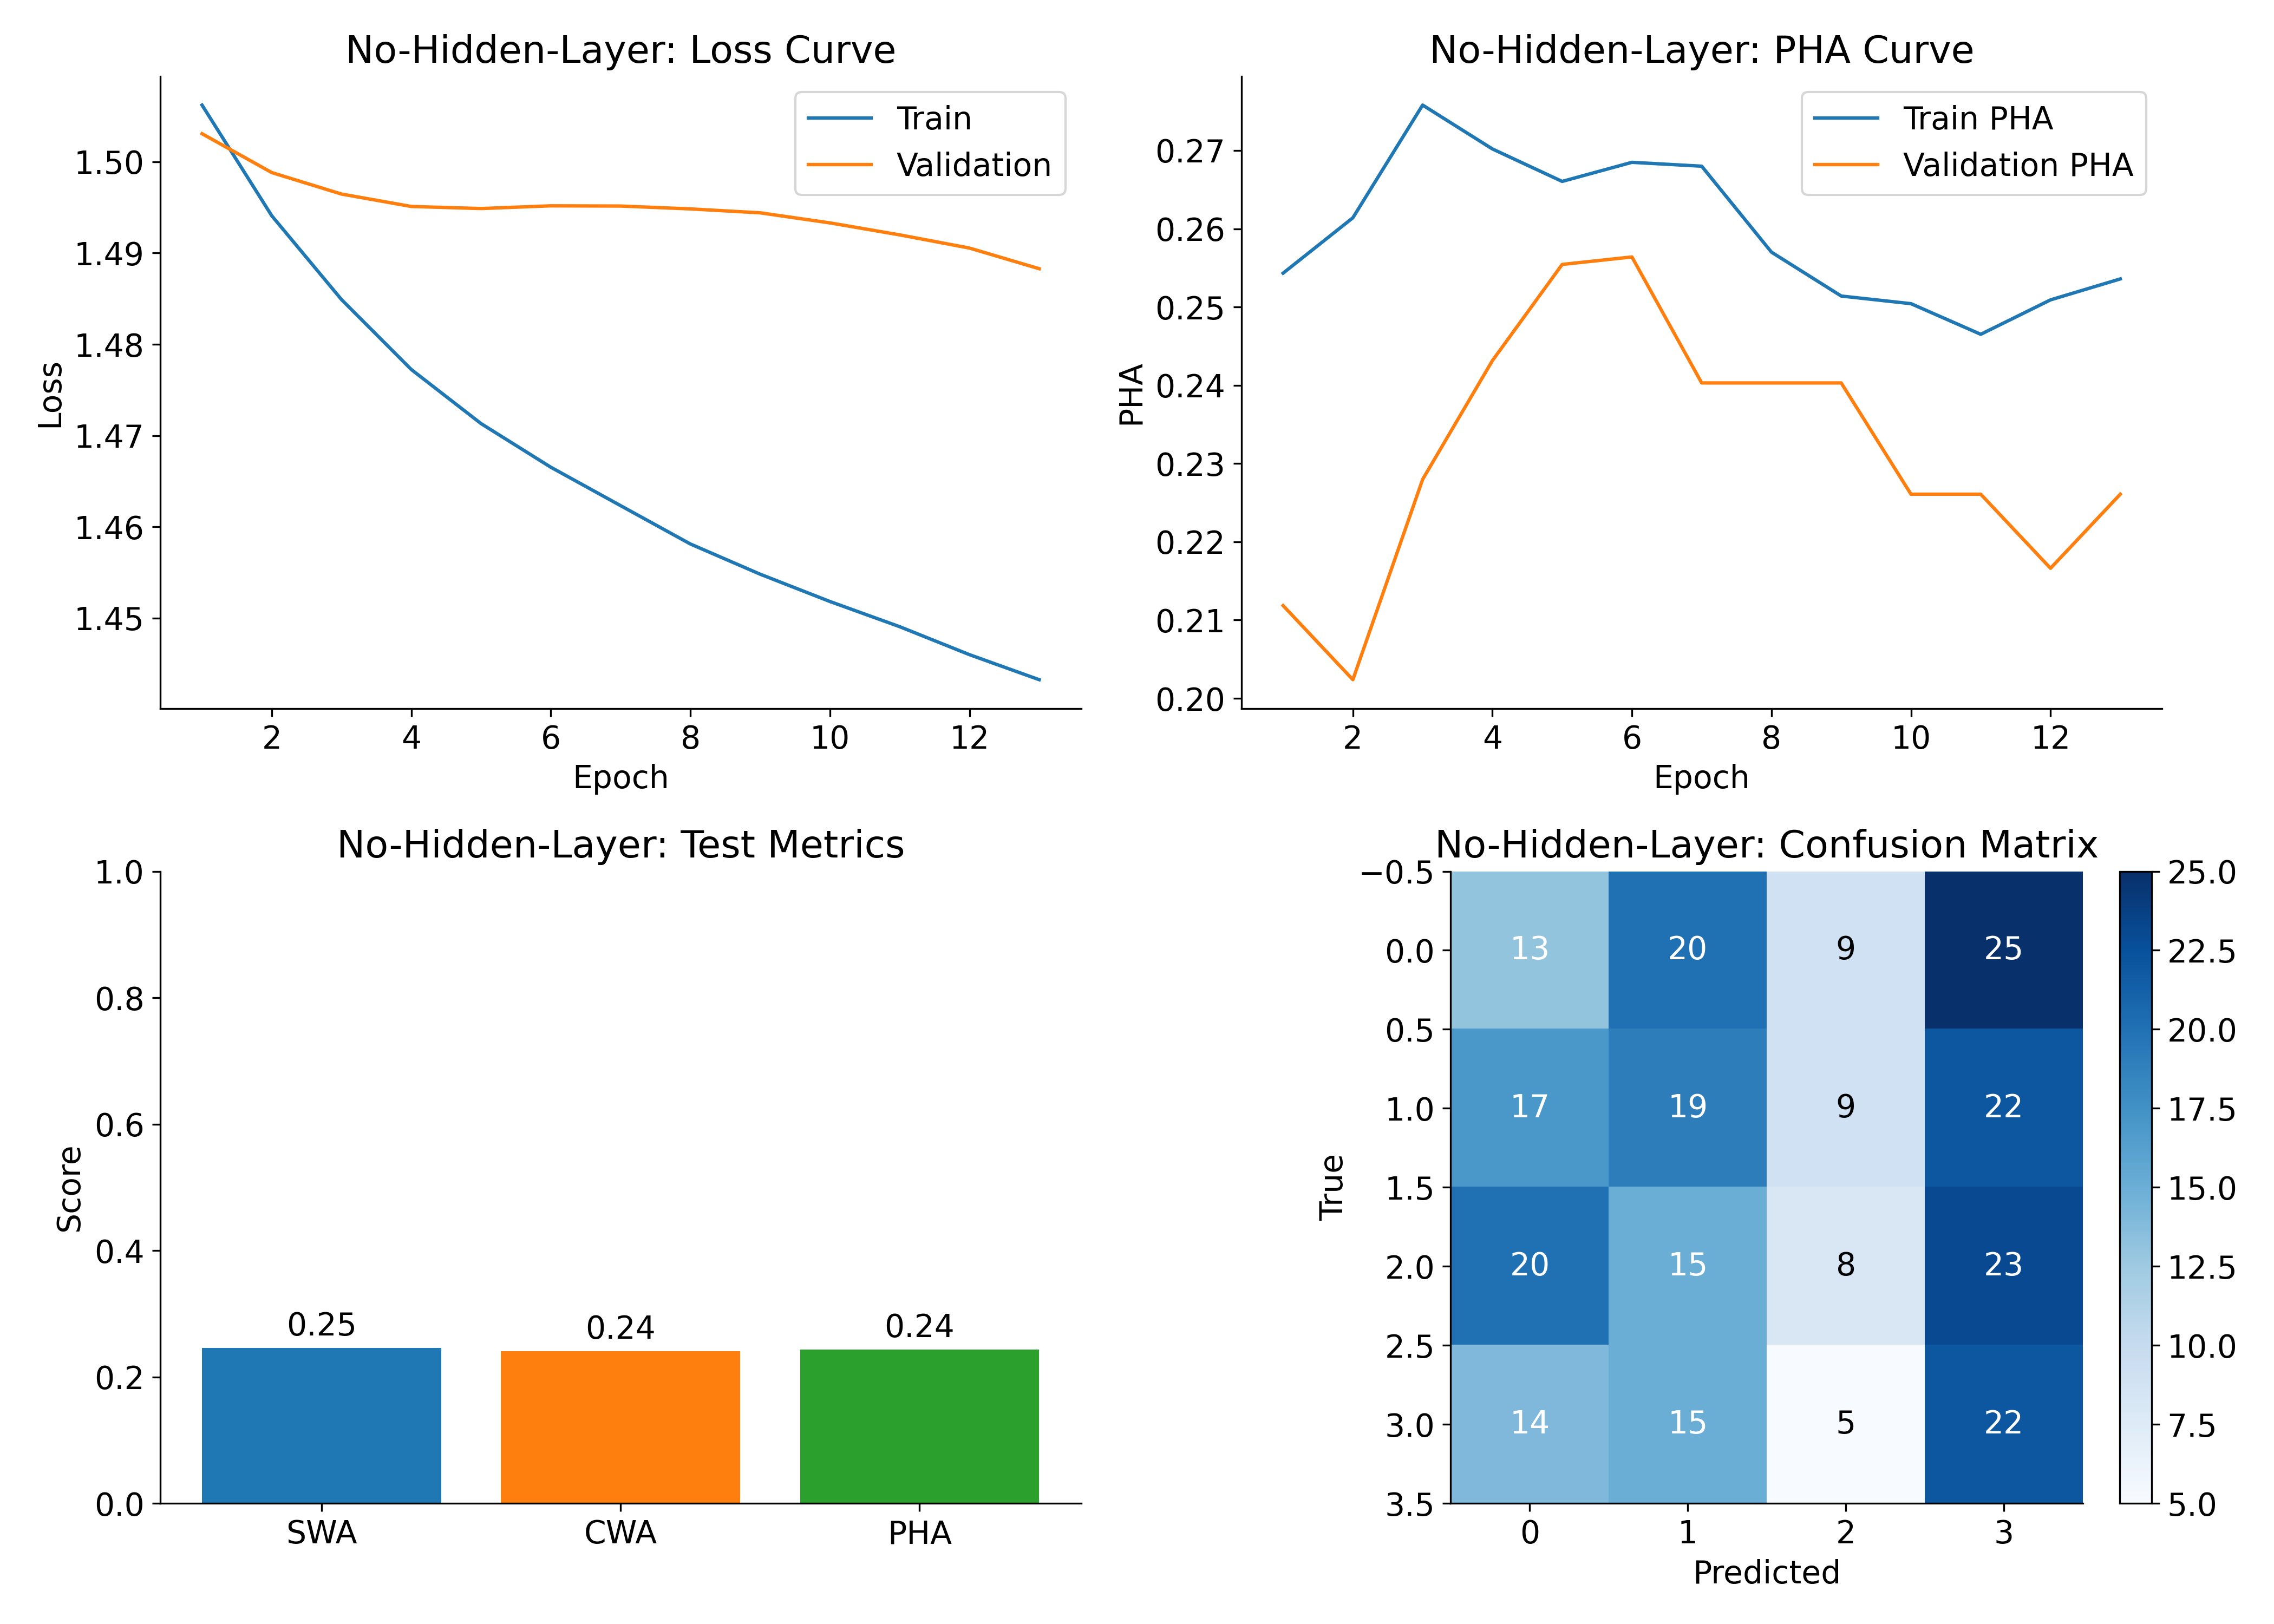
\includegraphics[width=0.6\textwidth]{no_hidden_layer_combined.png}
\caption{Using a linear-only model did not enhance generalization, indicating that reducing model complexity does not address overfitting.}
\label{fig:no_hidden_layer}
\end{figure}

\section{Experimental Details}
\label{sec:experimental_details}

\subsection{Hyperparameters}

The neural network component is a two-layer MLP with the following configuration:

\begin{itemize}
    \item \textbf{Input Size}: Variable, depending on the encoding of the input sequences.
    \item \textbf{Hidden Layer Size}: 128 neurons with ReLU activation.
    \item \textbf{Output Layer}: Softmax activation for classification.
    \item \textbf{Optimizer}: Adam with a learning rate of $1 \times 10^{-3}$.
    \item \textbf{Batch Size}: 32.
    \item \textbf{Epochs}: Trained up to 50 epochs with early stopping based on validation PHA.
\end{itemize}

\subsection{Data Preprocessing}

Each sequence in the dataset is composed of symbols with shape and color attributes. We encode shapes and colors using one-hot encoding and concatenate them to form the feature vectors for each symbol. The sequences are zero-padded to a fixed length for batch processing.

\section{Discussion}
\label{sec:discussion}

Our experiments consistently demonstrate that traditional neural networks struggle with zero-shot learning in the SPR domain. The overfitting observed suggests that the models memorize training data rather than learning generalizable rules. This behavior is problematic for applications requiring adaptability to unseen scenarios.

These findings align with those of \citet{hu2023codepa}, who highlight the importance of integrating neural models with symbolic components for complex reasoning tasks. The inability of the neural network to capture the compositional and rule-based nature of SPR indicates a mismatch between the neural architecture's capabilities and the requirements of the task.

Potential avenues for improvement include incorporating explicit rule induction mechanisms, leveraging attention-based architectures, or integrating external symbolic knowledge bases. Exploring alternative architectures that can effectively handle sequential and symbolic data might also improve generalization in SPR tasks.

Further research is necessary to develop models capable of effective zero-shot reasoning in complex symbolic domains like SPR.

\end{document}